% !TEX program = xelatex
% 本文是可持续更新的研究工作稿，而非某一具体期刊的排版终稿。
% 在 VS Code 中打开本文件，用 LaTeX Workshop 的 Build / View PDF 即可。
\documentclass[UTF8,fontset=none,zihao=-4,a4paper]{ctexart}
\setCJKmainfont{Songti SC}
\setCJKsansfont{PingFang SC}
\setCJKmonofont{Songti SC}
\usepackage[margin=2.35cm]{geometry}
\usepackage{amsmath,amssymb,booktabs,array,graphicx,float,caption,subcaption}
\usepackage{siunitx}
\usepackage{hyperref}
\usepackage{microtype}
\usepackage{enumitem}
\usepackage{needspace}
\usepackage{fancyhdr}
\hypersetup{colorlinks=true,linkcolor=black,citecolor=blue,urlcolor=blue,
  pdftitle={低统计量条件下基于散射角约束与自适应体素的缪子散射成像研究}}
\sisetup{detect-all}
\graphicspath{{figures/}}
\captionsetup{font=small,labelfont=bf}
\setlength{\parindent}{2em}
\setlength{\parskip}{0.15em}
\linespread{1.26}
\setlength{\headheight}{15pt}
\pagestyle{fancy}
\fancyhf{}
\fancyhead[L]{低统计量缪子散射成像研究工作稿}
\fancyhead[R]{\thepage}
\renewcommand{\headrulewidth}{0.3pt}

\title{低统计量条件下基于散射角约束与自适应体素的缪子散射成像研究\\\large 基于 Geant4 仿真与 POCA 重建的工作稿}
\author{作者姓名、单位与导师信息待补充}
\date{2026 年 9 月\quad 研究工作稿，尚未投稿}

\begin{document}
\maketitle
\begin{abstract}
针对缪子散射成像在有限事件数下轮廓不完整、定位不稳定的问题，本文建立了四层位置探测器与铝制 U 型目标的 Geant4 仿真系统，并以双直线最近点中点构造 POCA 散射位置。在理想 \SI{4}{GeV} 平行缪子源下，对获得完整四层击中的 \num{9975} 条事件进行固定 $32^3$ 体素重建；随后研究输入事件数、散射角筛选与截断加权、粗到细局部体素细分及位置测量误差。固定体素基线在 \num{1000}、\num{5000} 和 \num{9975} 条输入事件下的等面积 IoU 分别为 $0.2836$、$0.5916$ 和 $0.8409$。对于 \num{5000} 条输入事件，\SI{2}{mrad} 散射角下限与 \SI{3}{mrad} 权重截断把固定细体素的 IoU 提高至 $0.6324$；在相同筛选与权重设置下，以 $16^3$ 粗体素统计并细分得分最高的 $40\%$ 候选粗体素，IoU 为 $0.7234$。在五个 U 型场景的非零击中位置误差条件下，多数通过规则相对硬筛选的配对平均 IoU 增益为 $0.0234$，但自动窗口定位未同步改善。为检验形状迁移，固定所有规则后另以 L 型铝目标作留出验证；\num{5000} 条输入事件、$\sigma=\SI{0.05}{mm}$ 时，粗 $16^3$ 与 $40\%$ 细分的 IoU 分别为 $0.5975$ 与 $0.5095$，与无误差条件下两者的排序相反。结果提示固定细分比例对几何形状和击中误差敏感，轮廓与定位应分别评价。这些均为受控仿真结果，尚不能推广为真实宇宙线测量或跨材料、跨装置性能结论。
\end{abstract}

\noindent\textbf{关键词：}缪子散射成像；POCA；低统计量；散射角截断；自适应体素；事件质量；目标定位

\section{引言}
天然宇宙线缪子具有较强穿透能力，其穿过物质时发生的多重库仑散射可以提供被测区域内部结构信息。早期研究展示了利用宇宙线缪子进行无源成像的可行性\cite{borozdin2003}；后续工作系统讨论了散射角、散射位置和材料差异在重建中的作用\cite{schultz2004}。与通量充足的主动成像不同，缪子事件积累通常需要时间，因此有限事件数下的成像质量是值得单独研究的问题。

POCA（point of closest approach）将上下游拟合径迹的最近点对中点作为一次等效散射位置，计算过程直观、代价较低，但把沿路径分布的多次散射压缩为单点；在少量事件和测量噪声下，散射点位置以及角度权重都可能不稳定。本文的研究目标并非宣称用单一规则消除此类误差，而是建立一套可复现的分阶段比较：先量化固定体素基线的低统计量退化，再检验散射角约束和局部体素细分是否能在相同输入事件数下改善轮廓与定位，最后评估探测器误差对上述趋势的影响。

本文的研究贡献限于目前已有数据支持的范围：第一，构建 Geant4 四层探测器、U 型目标、事件 CSV、Python 重建及指标统计的完整链路；第二，以同一批事件子集比较固定体素、角度截断及粗细体素策略；第三，给出位置误差敏感性与简单不确定度修正的实验结果和适用边界；第四，对基于重复扰动的事件筛选与局部定位器作配对消融，并分析轮廓改善而定位恶化的失败样例；第五，固定 U 型场景中形成的参数，在未参与上述选择的 L 型铝目标上作跨形状检查。本文所用“自适应”是\emph{按粗体素散射分数排序并选择一部分细分}，尚不是学习得到的最优分辨率，也不是通用参数规律。留出 L 型测试只检验一种新形状，同材料、同装置、同理想源条件并未改变。

\section{仿真系统与事件数据}
\subsection{探测器、目标和坐标约定}
仿真使用 Geant4\cite{agostinelli2003}。坐标原点位于目标区域中心，名义缪子飞行方向为 $+z$。上游两层塑料闪烁体探测器中心位于 $z=-400$、$-300$\,mm，下游两层位于 $z=300$、$400$\,mm；同侧两层中心距 $d=100$\,mm。每层探测器的 $x,y$ 面半宽为 \SI{150}{mm}、$z$ 向半厚为 \SI{5}{mm}。当前事件记录采用理想化位置击中；探测效率、读出通道离散化和时间分辨尚未模拟。具体击中 $z$ 坐标可能是薄层的入射表面，而不是层中心，不应将层中心与 CSV 中击中位置混同。

中心场景的铝制目标由三个不重叠长方体拼成 U 形，$xy$ 外轮廓为 $120\times120$\,mm$^2$，壁厚 \SI{30}{mm}，沿 $z$ 方向厚 \SI{100}{mm}，开口朝向 $+y$。偏心场景把中心移至 $(25,-15)$\,mm；小目标场景为 $80\times80$\,mm$^2$、壁厚 \SI{20}{mm}。设置 U 形结构的目的，是同时考察位置、壁厚和空腔轮廓，而不是将其解释为某一真实工业样品。

跨形状留出验证另生成 L 型铝目标，由底边 $x\in[-60,60]$、$y\in[-60,-30]$\,mm 与左臂 $x\in[-60,-30]$、$y\in[-30,60]$\,mm 两个不重叠长方体组成；两者均沿 $z\in[-50,50]$\,mm 延伸。其外包络仍为 $120\times120$\,mm$^2$，壁厚仍为 \SI{30}{mm}，但去掉 U 型目标的右臂。因此这次仅构成目标形状变化，并非材料或厚度变化。L 型几何未用于前述角度门槛、细分比例与事件质量规则的选择。

\subsection{缪子源与数据筛选}
当前定量结果使用理想源：\SI{4}{GeV}、沿 $+z$ 方向入射。代码另外提供半自然入射开关，采用随机位置、简化角度分布及有限能量区间，但本文表格和主图\emph{未将其混入理想源结果}。这一模式不能替代经验证的海平面能谱和角分布。仿真事件通过四层探测器后，输出事件编号、四层击中位置以及由上下游轨迹得到的散射角和 POCA 坐标至 CSV；分析脚本仅保留具有四层完整击中的记录。本轮基线 CSV 含 \num{9975} 条完整事件，并不等同于总发射缪子数，也不等同于落入成像体积的 POCA 数。

成像区域为 $x,y\in[-90,90]$\,mm、$z\in[-100,100]$\,mm。使用全部 \num{9975} 条完整事件时，固定体素基线有 \num{1649} 个 POCA 点落在此成像范围内。需要指出，“输入事件数”“筛选后事件数”“范围内 POCA 数”分别对应不同处理阶段，本文均明确区分。

\section{重建方法}
\subsection{双直线径迹与散射角}
令两上游击中点为 $\mathbf a_1,\mathbf a_2$，两下游击中点为 $\mathbf b_1,\mathbf b_2$。定义入射和出射单位方向向量
\begin{equation}
\mathbf u_{\rm in}=\frac{\mathbf a_2-\mathbf a_1}{\|\mathbf a_2-\mathbf a_1\|},\qquad
\mathbf u_{\rm out}=\frac{\mathbf b_2-\mathbf b_1}{\|\mathbf b_2-\mathbf b_1\|}.
\end{equation}
总散射角可由两个方向向量夹角计算：
\begin{equation}
\theta=\arccos\!\left[\operatorname{clip}\!\left(\mathbf u_{\rm in}\cdot\mathbf u_{\rm out},-1,1\right)\right].
\label{eq:theta}
\end{equation}
实际数据字段另含 $x$、$y$ 方向的投影散射角；本文角度筛选与加权使用 CSV 中的 $\theta$，单位统一为 mrad。上下游各只有两层位置测量，因此直线由两点唯一确定，当前不能从每侧径迹拟合残差直接估计事件质量；若要使用残差，须增加测量层或独立约束。

\subsection{POCA 散射位置与固定体素基线}
两条径迹写成 $\mathbf r_{\rm in}(t)=\mathbf p+t\mathbf u_{\rm in}$ 与 $\mathbf r_{\rm out}(s)=\mathbf q+s\mathbf u_{\rm out}$。求使 $\|\mathbf r_{\rm in}(t)-\mathbf r_{\rm out}(s)\|$ 最小的一对参数 $t^*,s^*$，再取最近点对的中点作为 $\mathbf r_{\rm POCA}$。这只是单次等效散射近似；最近距离较大时还应结合探测器精度分析，而不能直接认定散射真实发生在该点。

固定体素基线将成像区域划分为 $32\times32\times32$ 个规则体素，体素 $v$ 的强度为
\begin{equation}
S_v^{\rm base}=\sum_{i:\mathbf r_{{\rm POCA},i}\in v}\theta_i^2.
\label{eq:baseline}
\end{equation}
三维体素沿 $z$ 轴求和，得到用于轮廓评价的 $xy$ 投影 $I_{xy}$。由于这里是角度平方\emph{求和}，图像强度同时受散射大小和局部计数影响；它不是经过材料厚度、动量或通量归一化的散射密度估计，也不应直接用于定量材料辨识。

\subsection{散射角筛选与截断加权}
角度约束只保留 $\theta_i\ge\theta_{\min}$ 的事件，并把每个保留事件的权重设为
\begin{equation}
w_i=\min\bigl(\theta_i^2,\theta_{\rm cap}^2\bigr),\quad
S_v^{\rm cap}=\sum_{i:\mathbf r_{{\rm POCA},i}\in v}w_i.
\label{eq:cap}
\end{equation}
本轮比较取 $\theta_{\min}=\SI{2}{mrad}$，扫描若干截断上限；后续粗细体素实验固定 $\theta_{\rm cap}=\SI{3}{mrad}$。设置下限是为减弱近直行事件的累积；上限是限制少数极端角度事件对平方权重的支配。这里的阈值是在当前数据场景中探索的候选值，不能不经验证就用于其他目标、动量谱或测量精度。

\subsection{粗到细的局部体素细分}
在相同事件与权重 $w_i$ 下，先用 $16^3$ 粗网格计算各粗体素 $c$ 的分数 $A_c=\sum_{i\in c}w_i$。脚本中细分候选的最小事件数实际为 $n_c\ge1$；按 $A_c$ 从大到小排序后，选取候选数的比例 $f\in\{0,0.1,0.2,0.3,0.4\}$。被选粗体素再划分为 $2\times2\times2$ 子体素，并按事件真实 POCA 落点重新累积；未选区域维持粗分辨率，但为统一评价，被均匀映射到对应的八个 $32^3$ 网格位置，总权重守恒。真值 U 型掩膜\emph{只用于后续评分}，不参加细分。

叶体素数量可写成 $16^3+7M$，其中 $M$ 为被细分的粗体素数。此处“自适应”的含义是\emph{基于观测分数的空间选择性细分}；固定比例 $f$ 仍是人工扫描参数。由于细分会改变局部平滑程度，其效果应同时与同一筛选条件下的固定 $32^3$ 细网格及完全不细分的 $16^3$ 粗网格比较，不能将所有增益笼统归因于“自适应”。

\subsection{基于击中扰动的事件质量估计}
对加入已知位置误差标准差 $\sigma$ 的四层测量击中，先重新求解名义轨迹、POCA 和式\eqref{eq:correction}所示的修正角；通过 $\theta_{\rm corr}\ge\SI{2}{mrad}$ 且满足现有成像筛选条件的事件构成共同的名义候选集 $\mathcal C$。在每条候选事件的\emph{同一测量击中}附近再独立施加 $K=12$ 次标准差为 $\sigma$ 的位置扰动，每次重新求轨迹与修正角。令 $m_i$ 为重新满足名义筛选条件的次数，定义经验通过频率 $p_i=m_i/K$。仅对通过的重算 POCA 坐标计算 $xy$ 平面均方根扩散 $s_i$；不足两次通过时按程序约定置 $s_i=0$。这种二次扰动是探测器误差敏感性探针，\emph{不是}严格的条件后验抽样或逐事件物理真值估计。

四个方案都从同一名义集合 $\mathcal C$ 出发，POCA 位置仍使用名义重建值。令名义截断角权重为 $w_i^0=\min(\theta_{{\rm corr},i}^2,\theta_{\rm cap}^2)$；$h=180/32=\SI{5.625}{mm}$ 为 $xy$ 细网格边长。实际使用的事件权重为
\begin{equation}
w_i^{(a)}=w_i^0\times\begin{cases}
1,&a=\mathrm{hard},\\
\mathbf 1[p_i\ge 0.5],&a=\mathrm{majority},\\
p_i,&a=\mathrm{pass\_prob},\\
p_i/[1+(s_i/h)^2],&a=\mathrm{pass\_spread}.
\end{cases}
\label{eq:quality}
\end{equation}
其中多数规则的阈值对应至少 6/12 次通过；连续规则分别表示通过频率加权、以及再按空间扩散降权。$h$ 来自既定重建网格，不由目标真值拟合。四组使用相同 $16^3\rightarrow32^3$、$40\%$ 候选细分设置。$\sigma=0$ 时四组构成一致性检查；当测量误差较大时，$p_i$ 不能消除 POCA 位置的系统漂移。目标真值仅在最终评分时使用，未进入事件权重或重建。

\section{实验设计与评价方法}
\subsection{低统计量抽样与对照}
从同一份理想源 CSV 中无放回抽取 \num{1000}、\num{3000}、\num{5000} 条完整事件，各重复 5 次；全量 \num{9975} 条只运行一次。基线脚本使用随机种子 \num{20260921}。角度与体素策略在各次重复中尽量使用相同输入子集作配对比较；其他独立鲁棒性实验的随机种子和事件处理可能不同，因此其绝对数值不与基线表直接做严格配对显著性推断。

\subsection{轮廓、定位与解释边界}
给定当前场景的真值二维掩膜 $T$（U 型或留出的 L 型），令 $k=|T|$；在重建投影 $I$ 中选强度最高的 $k$ 个像素作为预测掩膜 $P_k$，则等面积 IoU 定义为
\begin{equation}
\mathrm{IoU}=\frac{|P_k\cap T|}{|P_k\cup T|}.
\label{eq:iou}
\end{equation}
该指标固定了预测面积，便于比较图像空间位置和形状，但借用了仿真真值面积；真实未知目标不能直接采用此规则作为无监督分割器。定位误差使用\emph{整个 $xy$ 投影的散射强度加权质心}与真值掩膜几何质心的欧氏距离：
\begin{equation}
\mathbf c_I=\frac{\sum_{x,y}I_{xy}(x,y)(x,y)}{\sum_{x,y}I_{xy}(x,y)},\quad
e_{\rm loc}=\|\mathbf c_I-\mathbf c_T\|_2.
\label{eq:loc}
\end{equation}
它反映全局重心偏移，并不直接等同于目标检测框中心误差；一个边界错误但左右对称的图像，也可能有较小的 $e_{\rm loc}$。所有“均值$\pm$标准差”均为 5 次重复的描述统计，不应误读为独立装置重复测量所得的置信区间。目标/背景强度比与运行时间只作辅助观察；本稿不以尚未统一定义的 SSIM 或 MSE 代替上述主指标。

\subsection{事件质量配对与定位器消融设计}
在中心、偏心、小尺寸、中等偏移、小尺寸偏移五个 U 型铝目标场景中，每场景从四层完整击中记录抽取 $N\in\{1000,3000,5000\}$ 条事件，设置 $\sigma\in\{0,0.05,0.10,0.30\}$\,mm，每条件重复 5 次。每个 $(\text{场景},N,\text{重复},\sigma)$ 单元生成 hard、majority、pass\_prob、pass\_spread 四幅图；逐单元计算方法与 hard 的差，避免把不同随机子样本的绝对值直接相减。非零误差共有 $5\times3\times3\times5=225$ 个配对单元，零误差只作实现一致性检查。这里的重复来自模拟事件抽样和噪声随机数，不等于 225 次独立物理实验。

除全图质心外，使用同一张投影图像运行四个已实现且参数保持不变的定位器：全图强度质心、固定 $24\times24$ 网格滑窗、多尺度 $14/18/24$ 格候选滑窗、以及对正强度像素作第 95 百分位上限截断后的稳健多尺度滑窗。局部定位误差是\emph{选中窗口内估计中心}与真值掩膜几何中心的欧氏距离，不应与式\eqref{eq:loc}的全图质心误差混写。固定 24 格窗口依据当前目标最大尺度设定，包含尺度先验；它在未知尺寸目标上不一定公平。真值掩膜只参与最终误差计算，四个定位器均不读取真值。消融在 hard 与 majority 两类图像上逐图运行，既考察均值，也报告第 90 百分位误差（P90）和异常案例。

\subsection{L 型目标的留出验证协议}
在完成 U 型场景的方法探索后，保持相同四层探测器、\SI{4}{GeV} 理想平行源、成像范围、$\theta_{\min}=\SI{2}{mrad}$、$\theta_{\rm cap}=\SI{3}{mrad}$、$16^3\rightarrow32^3$ 网格、$40\%$ 细分比例及 $K=12$ 次事件扰动，不依据 L 型结果重新调参。独立 Geant4 运行发射 \num{10000} 个初级缪子，得到 \num{9976} 条四层完整击中；从该数据无放回抽取 $N\in\{1000,3000,5000\}$ 条，分别做 5 次抽样。四层的 $x,y$ 击中加入相同事件子集上成对复用的独立高斯误差，$\sigma\in\{0,0.05,0.10,0.30\}$\,mm。

每个条件重建七幅图：未筛选的固定 $32^3$ POCA（raw）、相同角度修正与筛选下的固定 $32^3$（hard fixed）、完全粗 $16^3$（hard coarse）、$40\%$ 局部细分（hard adaptive），以及在同一局部细分设置下的 majority、pass\_prob、pass\_spread。固定粗网格映射到 $32^3$ 后按相同等面积 Top-k 规则评分；L 型真值掩膜仅参与评分与事后图像叠加，不参与事件、体素或窗口选择。L 型场景的每种方法共 60 幅图；剔除 $\sigma=0$ 后，针对每一种对照有 $3\times3\times5=45$ 个逐条件配对单元。这些单元共享同一 Geant4 样本，不等于 45 次独立物理实验。

\section{实验结果}
\subsection{固定体素 POCA 的低统计量退化}
表\ref{tab:baseline}取自基线汇总 CSV。随着输入事件数增加，等面积 IoU 明显上升；\num{1000} 条下定位误差的重复间波动也较大。全量数据的 IoU 为 $0.8409$，但只做一次重建，没有误差条；它也不能与 5 次抽样结果按相同统计精度解读。

\begin{table}[htbp]
\centering
\caption{理想源下固定 $32^3$ 体素 POCA 基线。事件数是完整四层击中的输入条数。}
\label{tab:baseline}
\begin{tabular}{rrrrr}
\toprule
输入事件数 & 重复次数 & 范围内 POCA 数 & 等面积 IoU & 定位误差 / mm\\
\midrule
\num{1000} & 5 & $164.6\pm17.7$ & $0.2836\pm0.0256$ & $9.46\pm6.05$\\
\num{3000} & 5 & $499.8\pm16.5$ & $0.3802\pm0.0229$ & $7.13\pm4.77$\\
\num{5000} & 5 & $827.6\pm10.5$ & $0.5916\pm0.0202$ & $4.36\pm1.52$\\
\num{9975} & 1 & 1649 & 0.8409 & 3.80\\
\bottomrule
\end{tabular}
\end{table}

\begin{figure}[htbp]
\centering
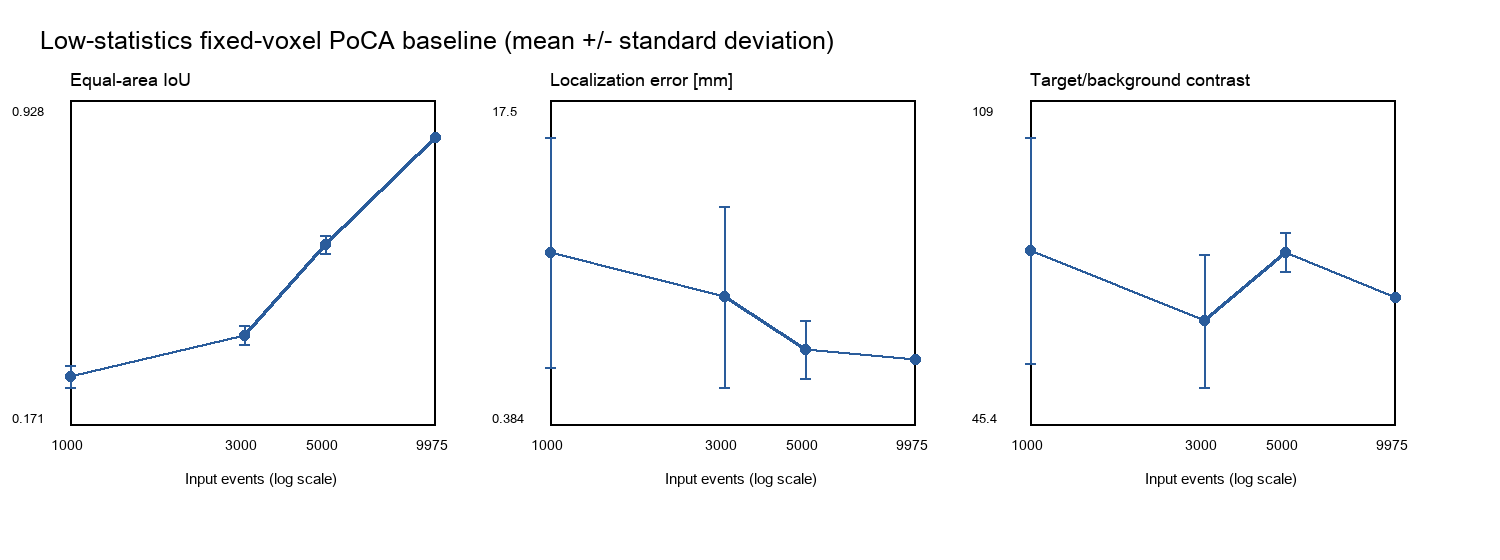
\includegraphics[width=0.86\linewidth]{baseline_metrics_vs_event_count.png}
\caption{固定体素 POCA 随输入事件数变化的评价指标；误差条对应重复抽样的标准差。图像由项目现有分析脚本生成。}
\label{fig:baseline}
\end{figure}

\subsection{角度筛选和截断权重的作用}
在 \num{5000} 条输入事件下，$\theta\ge\SI{2}{mrad}$ 使平均保留事件数为 559.0，真正落在成像体积内的平均 POCA 数为 410.8。$\theta_{\rm cap}=\SI{3}{mrad}$ 时，固定 $32^3$ 网格的 IoU 为 $0.6324\pm0.0178$，定位误差为 $1.59\pm0.45$\,mm，优于同数据基线的 $0.5916\pm0.0202$ 与 $4.36\pm1.52$\,mm。上限为 \SI{2}{mrad} 时 IoU 略高（$0.6342$），但定位误差为 $1.61$\,mm；两者差距很小，不应声称 \SI{3}{mrad} 在所有指标上唯一最优。去掉权重上限后，IoU 仍约为 $0.6316$，但定位误差升至 $4.70$\,mm，说明极端权重对重心可能更敏感。

\begin{figure}[htbp]
\centering
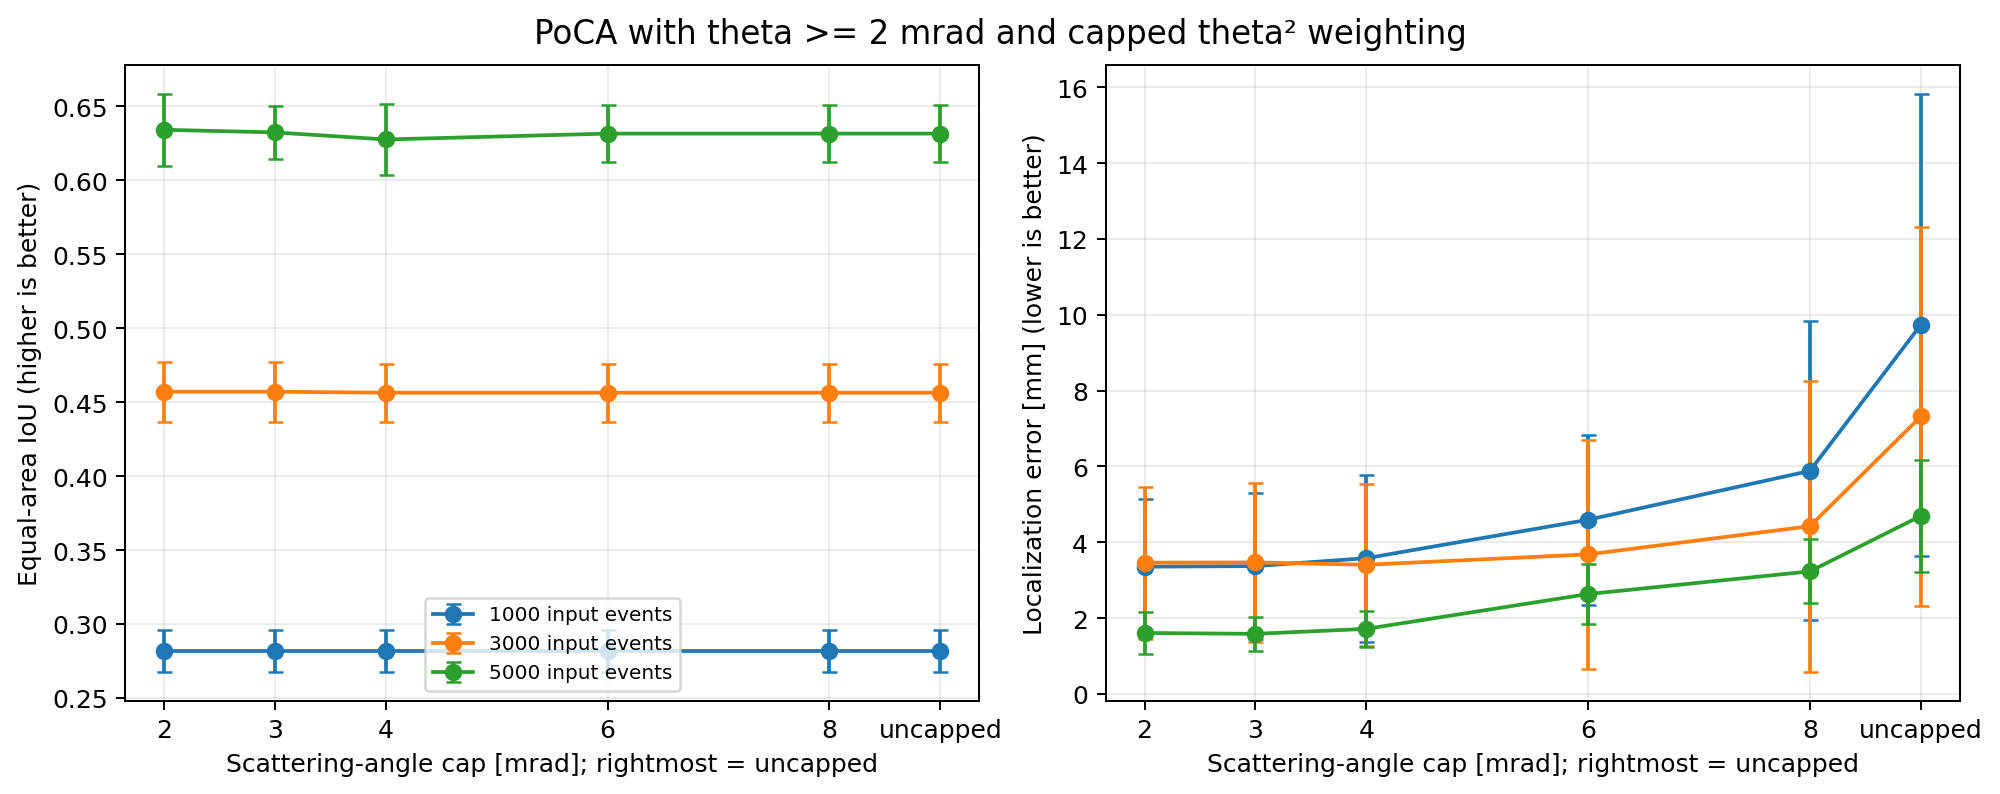
\includegraphics[width=0.86\linewidth]{angle_weighting_metrics_vs_cap.png}
\caption{固定角度下限 \SI{2}{mrad} 时，不同角度平方权重截断上限的性能对比。横向比较必须同时查看 IoU 和定位误差。}
\label{fig:angle}
\end{figure}

\subsection{粗网格及局部细分的比较}
表\ref{tab:adaptive}同时列出未筛选固定网格、同一角度筛选条件下的固定细网格，以及粗到细策略。\num{5000} 条输入事件时，完全不细分的 $16^3$ 粗网格已得到 $0.6693$ 的 IoU；将 $40\%$ 候选粗体素细分后升至 $0.7234$，相应定位误差约 $1.45$\,mm。因而与未筛选基线相比的增益由\emph{事件约束、粗网格平滑与局部细分}共同造成；在同筛选条件内，局部细分相对纯粗网格的 IoU 增益约 $0.0541$。\num{3000} 条事件下，完全不细分的粗网格 IoU 为 $0.6531$，提醒我们低统计量时过度细分可能并不有利。当前并没有对 $f$ 做外部场景独立选择，因此不能把 $40\%$ 宣称为普适最优比例。

\begin{table}[htbp]
\centering
\caption{中心 U 型目标的代表性对比。各行的筛选和网格条件应一并阅读，不能把不同处理阶段视为单变量比较。}
\label{tab:adaptive}
\begin{tabular}{p{0.50\linewidth}rr}
\toprule
方法及输入事件数 & 等面积 IoU & 定位误差 / mm\\
\midrule
\num{3000}，固定 $32^3$，未筛选 & $0.3802\pm0.0229$ & $7.13\pm4.77$\\
\num{3000}，固定 $32^3$，角度筛选+截断 & $0.4571$ & $3.47$\\
\num{3000}，粗 $16^3$，$f=0$ & $0.6531$ & $3.39$\\
\num{5000}，固定 $32^3$，未筛选 & $0.5916\pm0.0202$ & $4.36\pm1.52$\\
\num{5000}，固定 $32^3$，角度筛选+截断 & $0.6324\pm0.0178$ & $1.59\pm0.45$\\
\num{5000}，粗 $16^3$，$f=0$ & $0.6693\pm0.0145$ & $1.44\pm0.41$\\
\num{5000}，粗到细，$f=0.4$ & $0.7234\pm0.0085$ & $1.45\pm0.50$\\
\bottomrule
\end{tabular}
\end{table}

\begin{figure}[htbp]
\centering
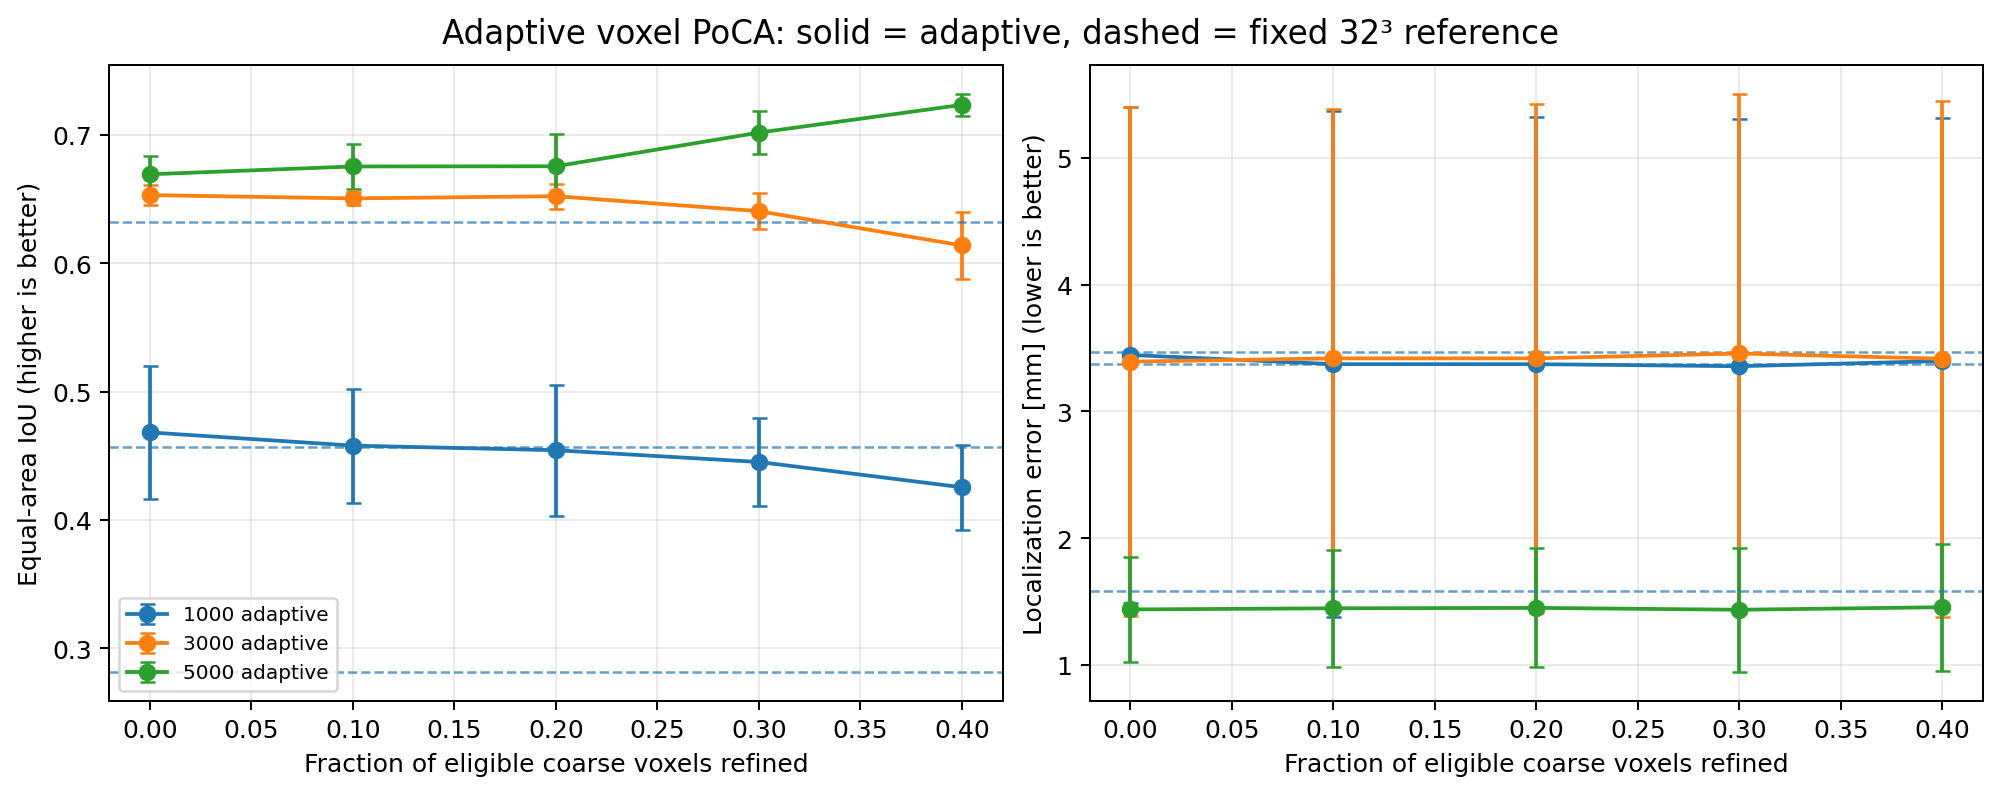
\includegraphics[width=0.85\linewidth]{adaptive_voxel_metrics_vs_refinement.png}
\caption{不同输入事件数下细分比例对 IoU 和定位误差的影响。图中虚线是相同筛选条件下的固定细体素参考。}
\label{fig:adaptive}
\end{figure}

\subsection{位置和尺度变化下的辅助验证}
为检验结论是否只来自中心大目标，还分别运行偏心 U 型和小尺寸 U 型场景。表\ref{tab:scenario}只比较各场景内、\num{5000} 条输入事件时的相同角度筛选与截断设置，且每行均为 5 次重复均值。偏心目标中，完全不细分的粗网格 IoU 最高；小目标中，固定细网格略高于粗到细策略。由此可见，中心场景的 $40\%$ 细分比例不能直接推广为跨位置、跨尺度的统一最优规则。更可取的后续目标是根据局部计数与图像尺度选择分辨率，同时在未参与参数选择的场景上报告结果。

\begin{table}[htbp]
\centering
\caption{不同 U 型场景的辅助验证。数值为等面积 IoU 的 5 次重复均值；同一行对照均使用相同角度筛选与权重上限。}
\label{tab:scenario}
\begin{tabular}{lrrr}
\toprule
场景 & 固定 $32^3$ & 粗 $16^3$，$f=0$ & 粗到细，$f=0.4$\\
\midrule
中心 $120$\,mm U 型 & 0.6324 & 0.6693 & 0.7234\\
偏心 $120$\,mm U 型 & 0.6121 & 0.7458 & 0.7276\\
中心 $80$\,mm U 型 & 0.5978 & 0.5527 & 0.5825\\
\bottomrule
\end{tabular}
\end{table}

\Needspace{8\baselineskip}
\subsection{击中位置误差与不确定度修正}
为考察非理想位置测量，在四层击中的 $x$、$y$ 坐标分别加入独立零均值高斯误差，标准差记为 $\sigma$；随后重新计算轨迹、散射角与 POCA。独立的探测器分辨率实验显示，对 \num{5000} 条输入事件的 $40\%$ 细分策略，$\sigma=0$、$0.05$ 和 $0.10$\,mm 时，IoU 分别约为 $0.730$、$0.515$ 和 $0.349$。这是位置误差敏感性的证据，不能用“亚毫米误差可以忽略”概括。

\begin{figure}[htbp]
\centering
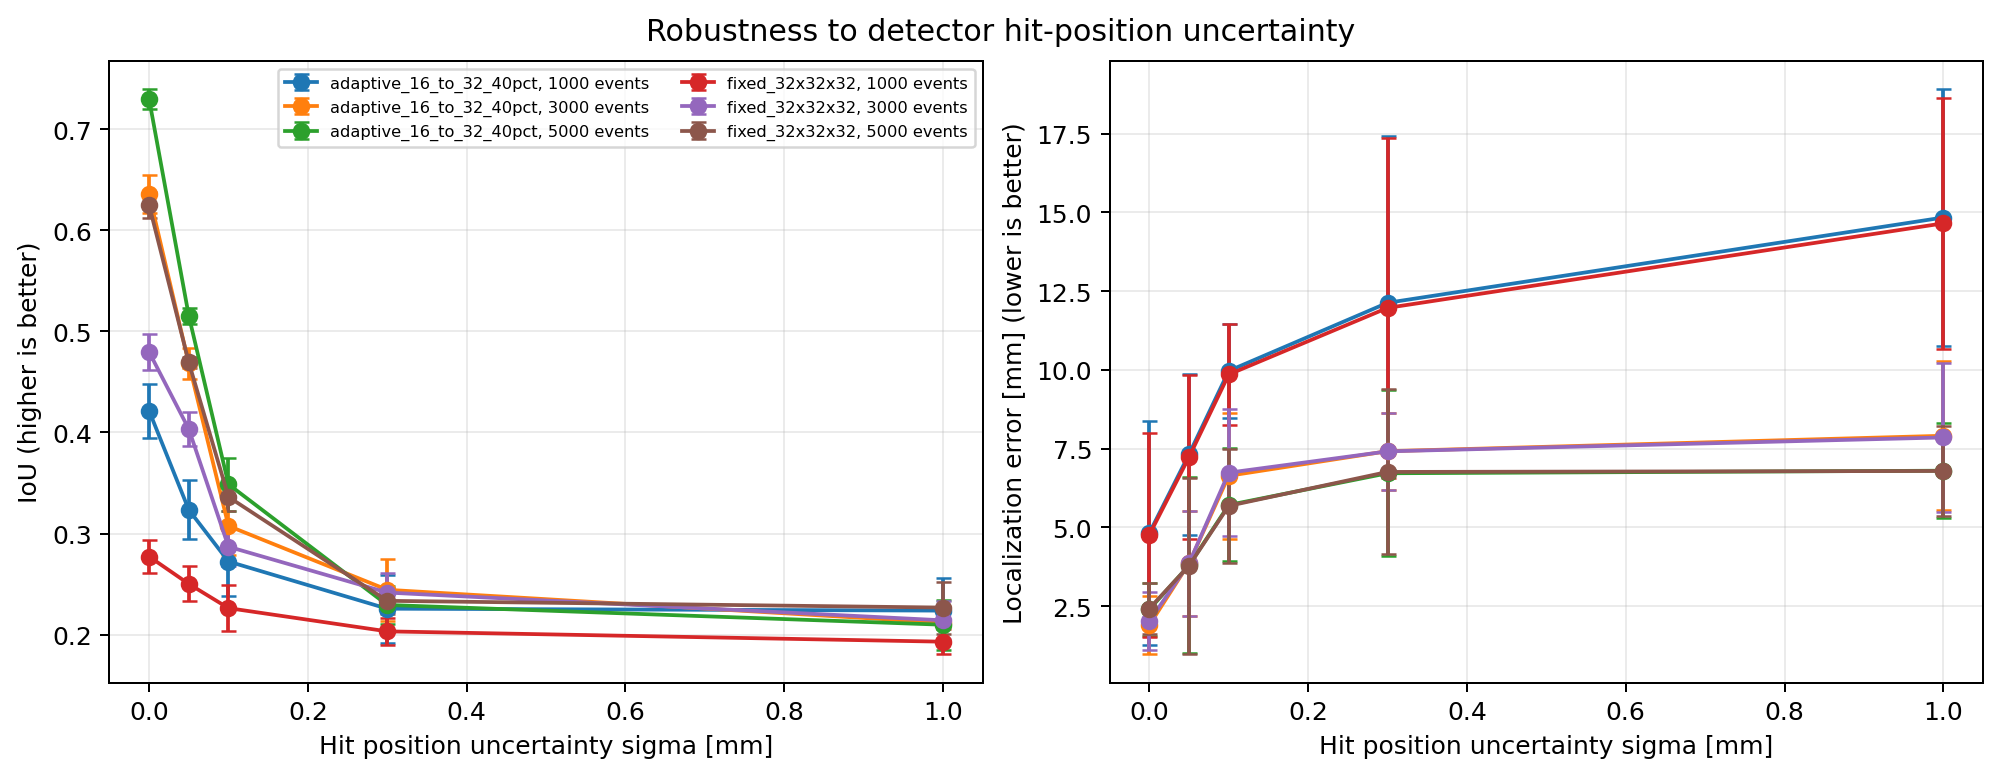
\includegraphics[width=0.86\linewidth]{detector_resolution_metrics.png}
\caption{探测器击中位置误差对重建的影响。该图来自独立的分辨率实验，不与图\ref{fig:uncertainty} 的均值直接作配对差异解释。}
\label{fig:resolution}
\end{figure}

同侧两层中心距为 $d$ 时，每层每坐标独立误差 $\sigma$ 在小角近似下导致一个投影散射角差的方差约 $4\sigma^2/d^2$；两个正交投影合起来，二维角度噪声平方的期望近似为 $8\sigma^2/d^2$。据此构造探索性的角度修正
\begin{equation}
\theta_{\rm noise}=\sqrt{8}\,\sigma/d,\qquad
\theta_{\rm corr}=\sqrt{\max\!\left(\theta_{\rm obs}^2-\theta_{\rm noise}^2,0\right)}.
\label{eq:correction}
\end{equation}
这是均方意义的简化扣除，而不是逐事件真实散射角的无偏估计；它没有修正因击中误差导致的 POCA 位置漂移，也忽略了能谱与多次散射分布的细节。$d=\SI{100}{mm}$、$\sigma=\SI{0.1}{mm}$ 时，$\theta_{\rm noise}\approx\SI{2.83}{mrad}$，已与所用 \SI{2}{mrad} 下限相近。

在同一组不确定度修正实验中，\num{5000} 条事件、$40\%$ 细分、$\sigma=\SI{0.05}{mm}$ 时，修正角与未修正观测角的 IoU 分别为 $0.5572$ 与 $0.5114$；$\sigma=\SI{0.10}{mm}$ 时分别为 $0.4000$ 与 $0.3531$。但在 $\sigma=\SI{1.0}{mm}$ 时，修正后的 IoU 为 $0.1745$，低于未修正的 $0.1830$；部分条件下定位误差也未同步变好。故结果只支持“中等误差下有改善迹象”，\emph{不支持}“简单扣除普遍有效”。

\begin{figure}[htbp]
\centering
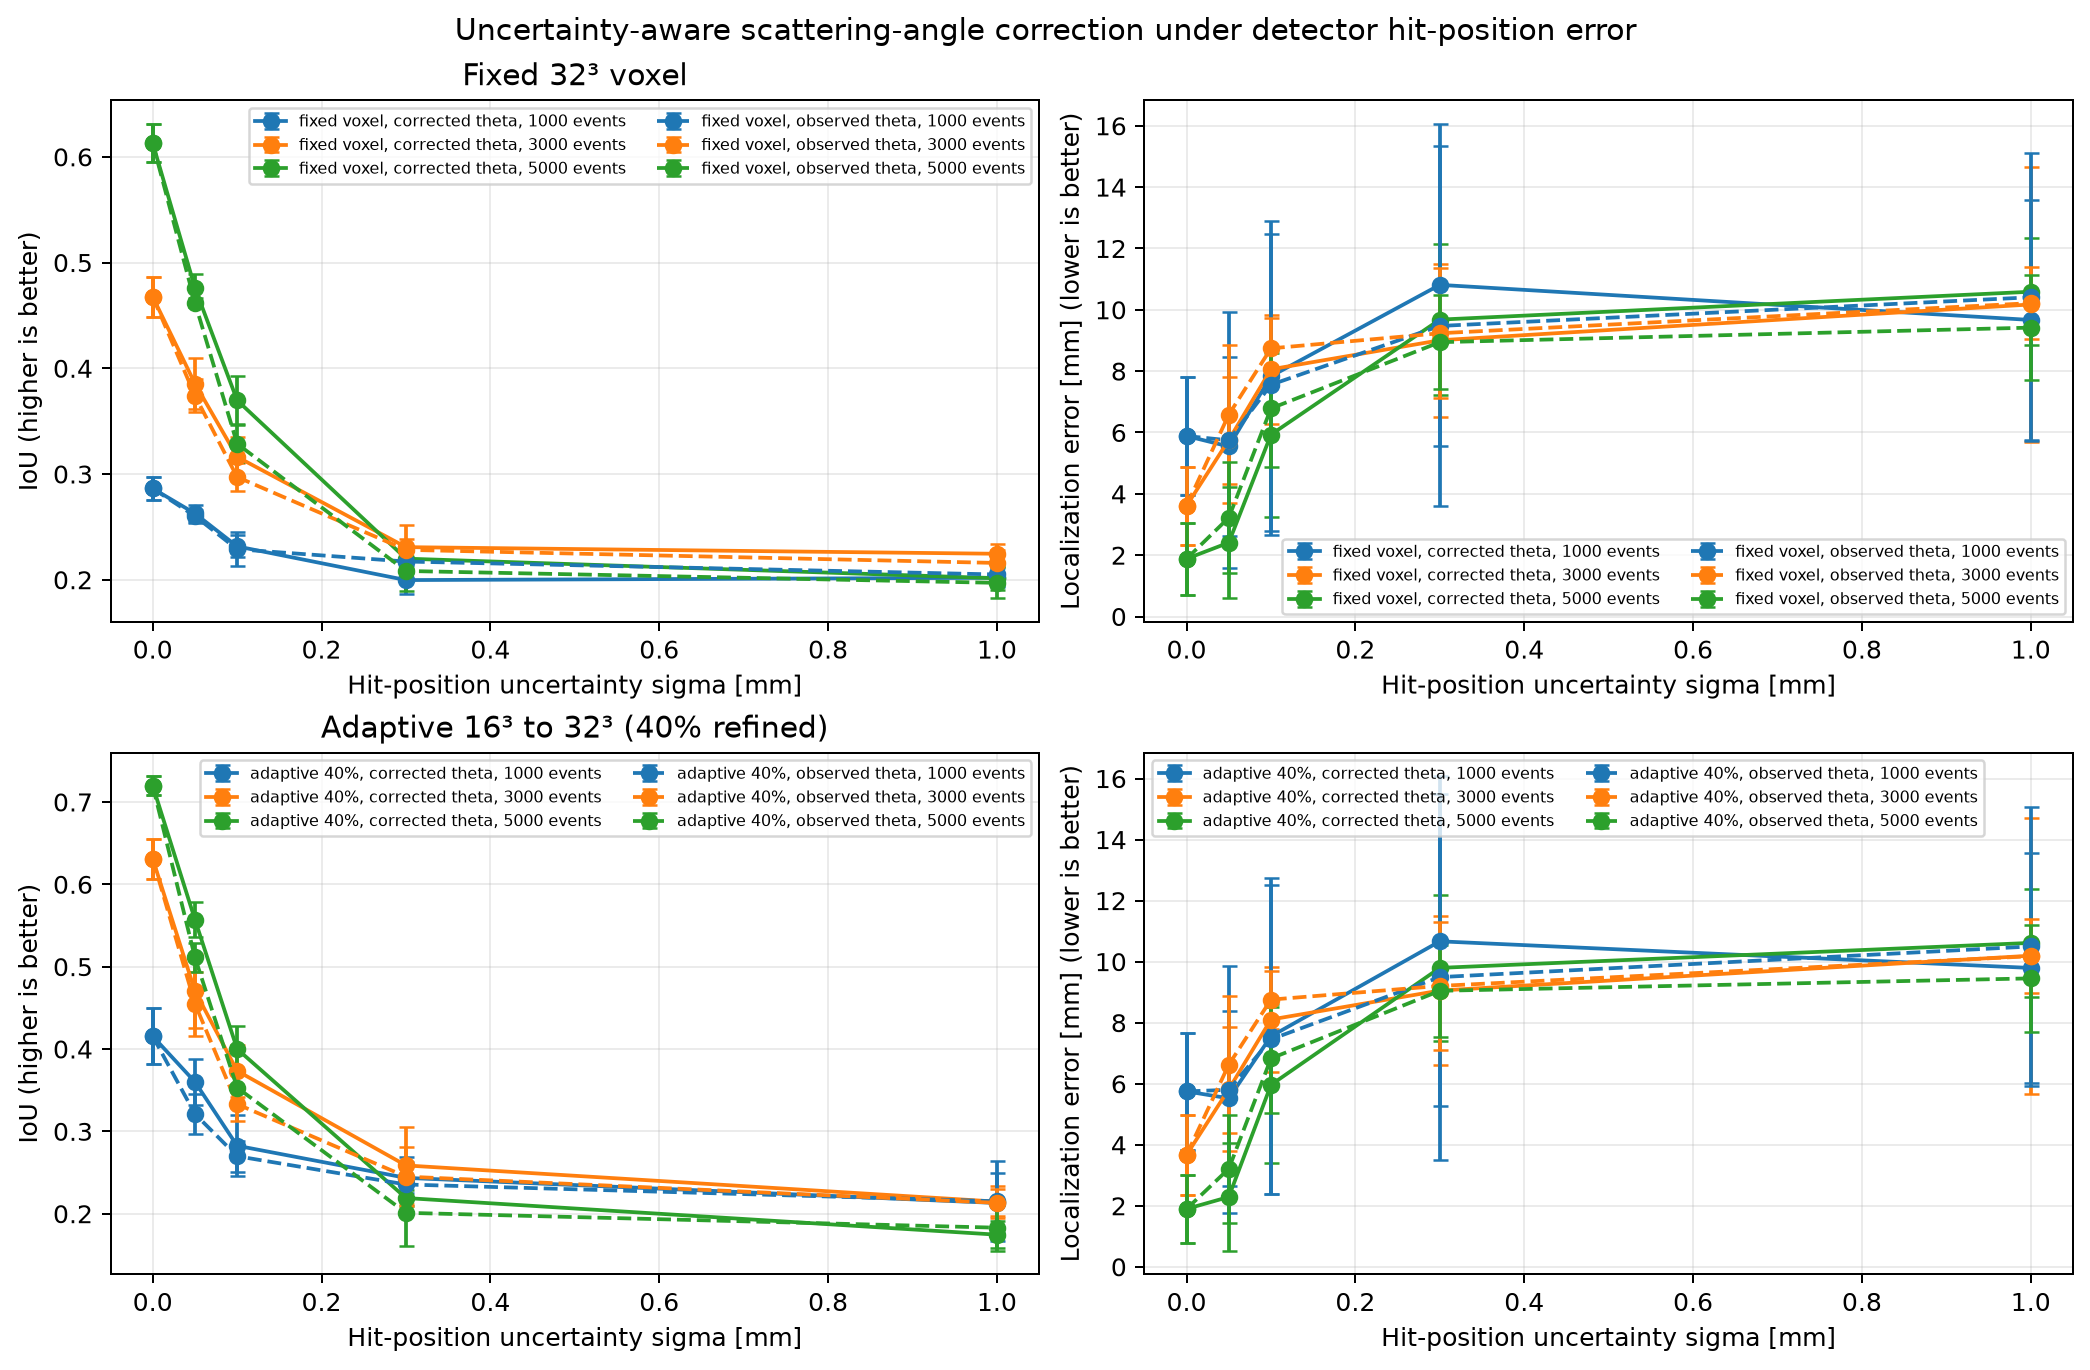
\includegraphics[width=0.95\linewidth]{uncertainty_aware_angle_metrics.png}
\caption{观测角与简化噪声扣除角在不同击中位置误差下的比较。上排为固定 $32^3$ 体素，下排为 $16^3\rightarrow32^3$、$40\%$ 细分；左列 IoU 越大越好，右列定位误差越小越好。}
\label{fig:uncertainty}
\end{figure}

\subsection{事件质量规则的配对比较}
为避免仅凭单个中心场景或单一指标判断方法优劣，表\ref{tab:quality}汇总 $\sigma>0$ 的 225 个配对单元。IoU 增益定义为 $\mathrm{IoU}_{a}-\mathrm{IoU}_{\rm hard}$；定位误差减少定义为 $e_{\rm hard}-e_a$，故正数表示改善。所有数值是跨五场景、三事件数、三非零误差水平和五重复的描述性平均，不附带独立样本显著性结论。

\begin{table}[htbp]
\centering
\caption{非零击中位置误差下事件质量策略相对 hard 的逐条件配对结果（225 单元）。自动窗口采用既有多尺度定位器。}
\label{tab:quality}
\small
\begin{tabular}{lrrrr}
\toprule
方法 & 平均 IoU 增益 & IoU 胜率 / \% & 全图误差减少 / mm & 自动窗口误差减少 / mm\\
\midrule
majority & $+0.0234$ & 70.2 & $+0.4009$ & $-0.0223$\\
pass\_prob & $+0.0014$ & 49.8 & $+1.1170$ & $+1.7611$\\
pass\_spread & $+0.0025$ & 48.0 & $+1.1104$ & $+1.0094$\\
\bottomrule
\end{tabular}
\end{table}

多数通过规则的轮廓收益最稳定，但多尺度自动窗口误差平均并未降低；两个连续权重方案的自动定位平均误差有下降迹象，却没有稳定的逐图 IoU 胜率。以 $N=5000$、$\sigma=\SI{0.10}{mm}$ 为例，majority 相对 hard 的平均 IoU 增益约为 $0.0354$，但自动窗口误差反而增加约 $1.47$\,mm。更高的 $\sigma=\SI{0.30}{mm}$ 下部分偏心或小目标场景出现负收益，故不存在本实验三个指标均占优的事件质量方案。图\ref{fig:paired}展示逐场景的权衡；图和表不能被解释为真实装置上的置信结论。

\begin{figure}[htbp]
\centering
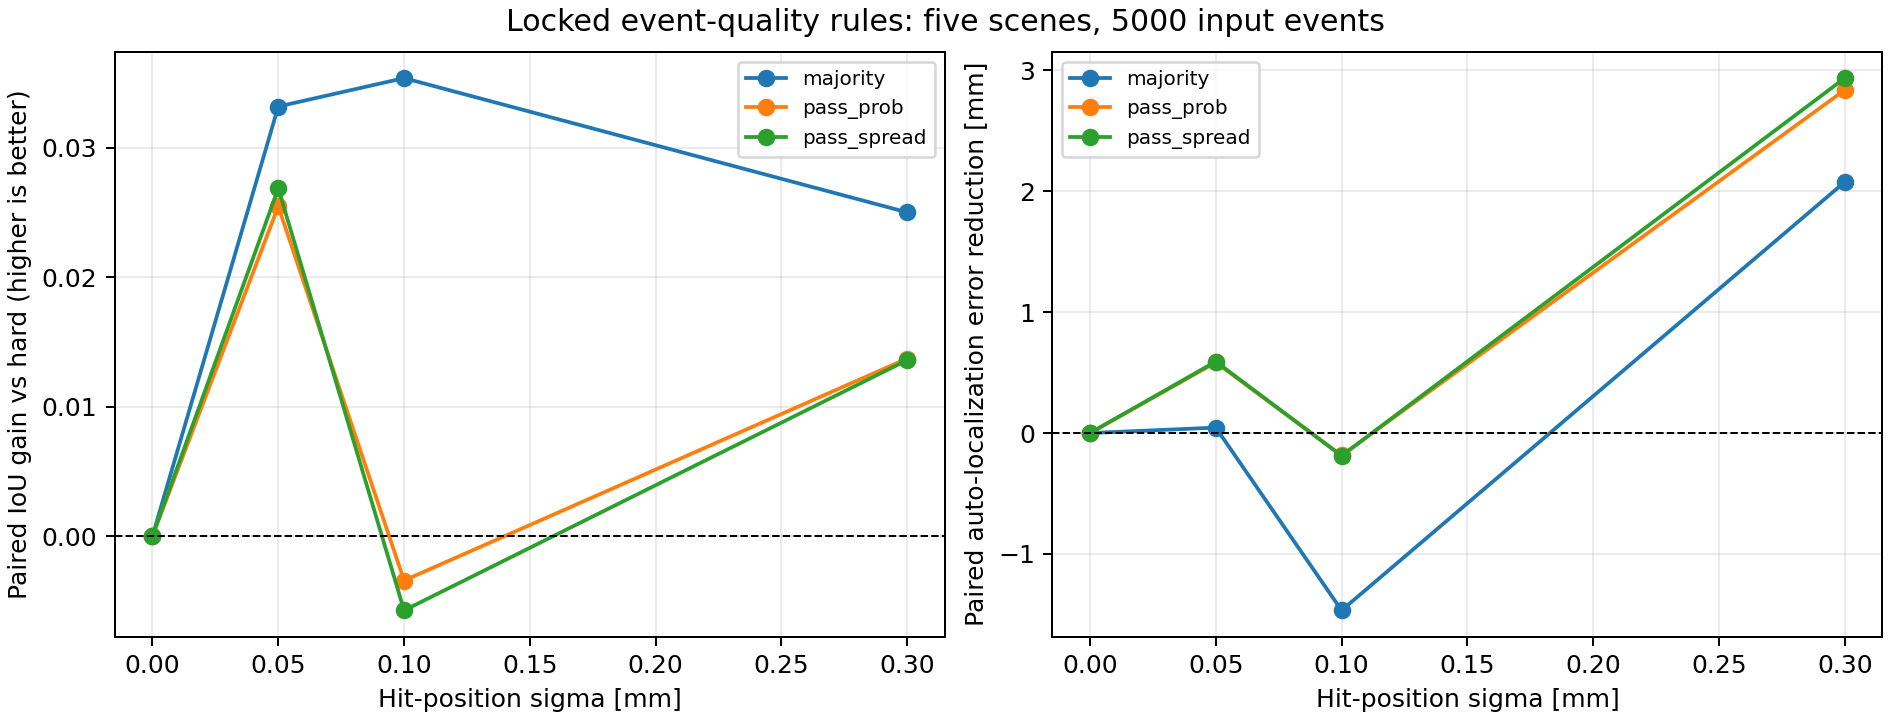
\includegraphics[width=0.9\linewidth]{paired_tradeoff_5000.png}
\caption{输入事件数 $N=5000$ 的五场景配对差异。轮廓与定位的增益方向分别按正文定义；不同误差水平与场景的符号变化提示平均数不能替代逐条件检查。}
\label{fig:paired}
\end{figure}

\subsection{定位器消融与失败案例}
在 hard 和 majority 各 225 张非零误差图像上，固定参数重放四种定位器，结果列于表\ref{tab:localizer}。固定 24 格窗口的平均误差和 P90 均低于本实验的多尺度窗口，但相对多尺度逐图胜率仅为 hard 的 $56.0\%$ 与 majority 的 $63.6\%$，并非逐例占优。稳健多尺度也未稳定解决大误差尾部。

\begin{table}[H]
\centering
\caption{非零击中位置误差下定位误差的描述统计，单位 mm；每类重建图像均为 225 张。P90 为误差的第 90 百分位数。}
\label{tab:localizer}
\small
\begin{tabular}{llrr}
\toprule
重建图 & 定位器 & 平均误差 & P90\\
\midrule
hard & 全图质心 & 13.34 & 28.37\\
hard & 固定 24 格窗口 & 14.40 & 31.82\\
hard & 多尺度窗口 & 20.81 & 56.04\\
hard & 稳健多尺度 & 20.87 & 53.89\\
majority & 全图质心 & 12.94 & 28.87\\
majority & 固定 24 格窗口 & 13.86 & 33.20\\
majority & 多尺度窗口 & 20.84 & 56.94\\
majority & 稳健多尺度 & 21.82 & 57.49\\
\bottomrule
\end{tabular}
\end{table}

\begin{figure}[H]
\centering
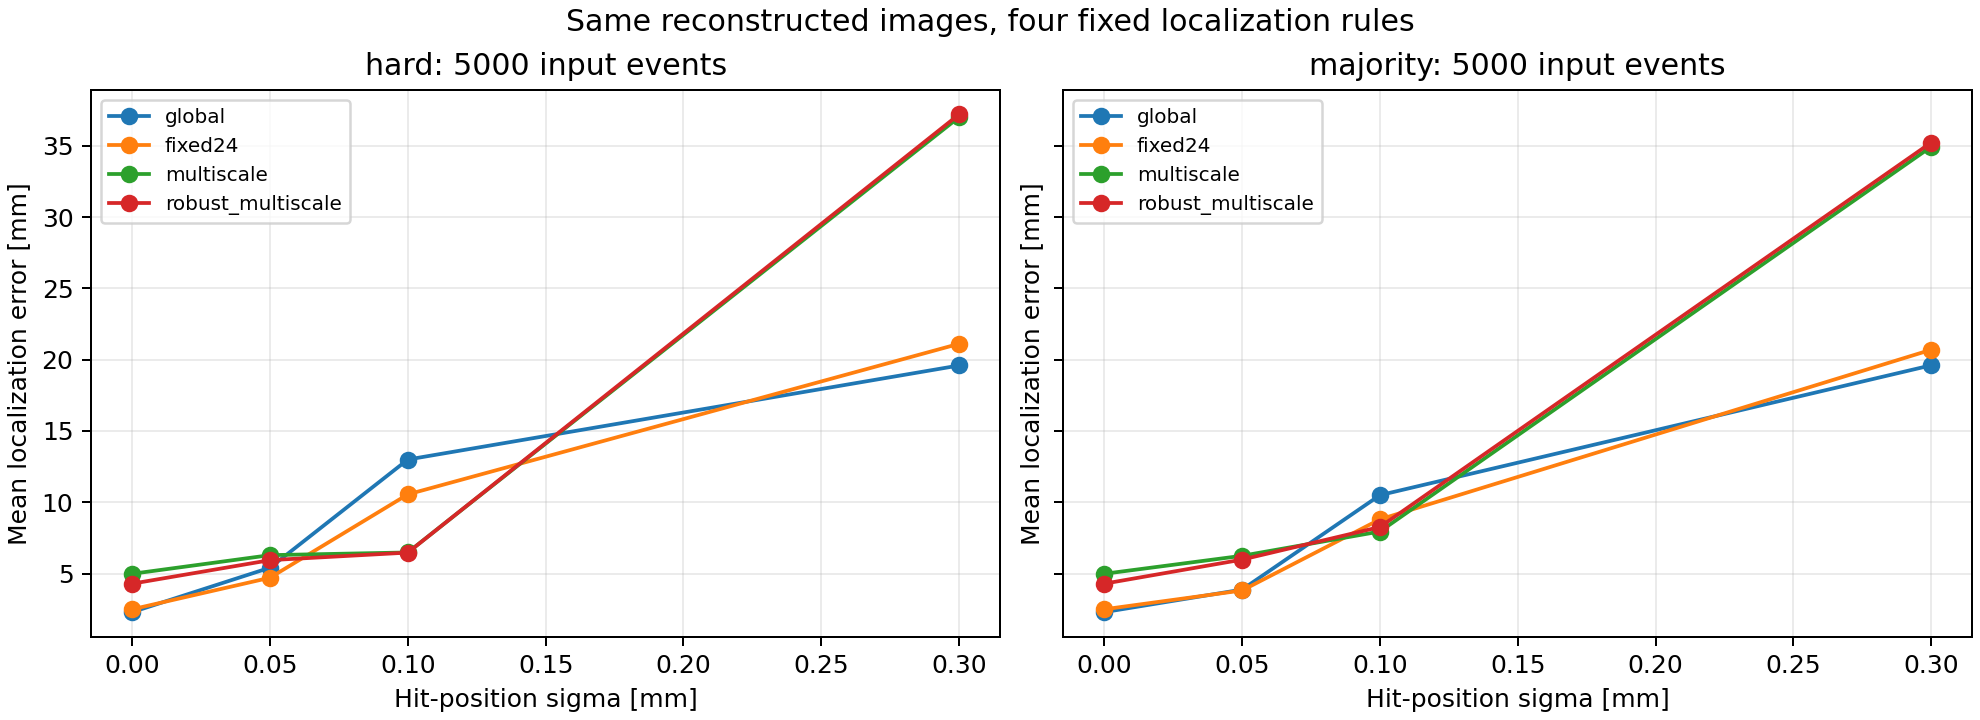
\includegraphics[width=0.80\linewidth]{localizer_ablation_5000.png}
\caption{$N=5000$ 条事件时不同定位器的误差对比。四种定位器在相同重建图像上运行；固定窗口所含目标尺度先验不可忽略。}
\label{fig:localizer}
\end{figure}

多尺度选中窗口触及成像边界时，hard 中有 $31/225$ 张图，平均误差 $43.72$\,mm，未触边的 194 张图平均 $17.15$\,mm；majority 中相应为 $23/225$ 张图、$42.80$\,mm，对比未触边 202 张图的 $18.33$\,mm。这是\emph{触边与高误差的关联}，不能证明触边是唯一原因，亦不能未经外部数据验证就加入后处理规则。

图\ref{fig:failure}为\emph{事后挑选}的诊断案例：偏心目标、$N=5000$、第 1 次重复、$\sigma=\SI{0.10}{mm}$。hard 到 majority 后，等面积 IoU 由 $0.384$ 升至 $0.456$，全图质心误差由 $15.35$ 降至 $7.33$\,mm，目标掩膜内权重占比由 $0.531$ 升至 $0.641$；然而多尺度窗口从 18 格、起点 $(13,2)$ 改为 14 格、起点 $(17,2)$，局部定位误差由 $17.54$ 升至 $34.10$\,mm。相同 majority 图像的固定 24 格定位误差为 $3.49$\,mm。图像相对更集中于真实目标并不保证局部窗口覆盖完整 U 型：局部热点可能使窗口收缩或偏向单侧 U 臂。另一个高噪声小目标案例中，$N=3000$、$\sigma=\SI{0.30}{mm}$ 时，majority 的 IoU 仅由 $0.054$ 到 $0.064$，多尺度定位误差由 $5.88$ 增至 $64.45$\,mm；即使换固定 24 格窗口，误差仍有 $39.95$\,mm，说明图像信息不足时换窗口不能完全补救。所列个案只用于解释机制，\emph{不是}对新定位方法的独立验证。

\begin{figure}[htbp]
\centering
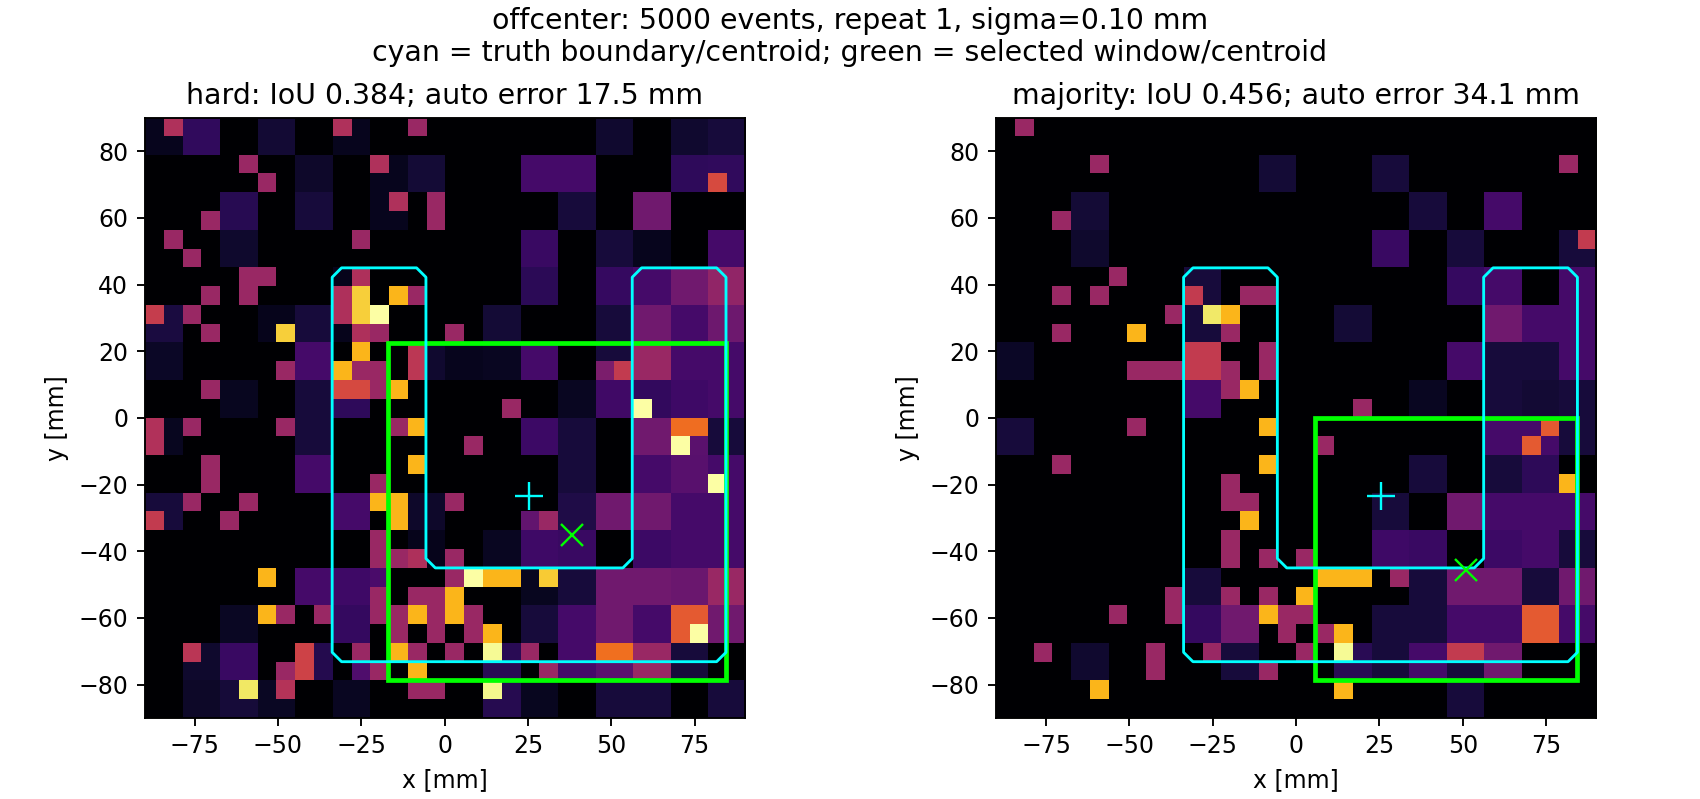
\includegraphics[width=0.93\linewidth]{offcenter_5000_r1_sigma0.10.png}
\caption{偏心 U 型场景的事后失败诊断：相同事件与误差条件下，majority 改善轮廓和全图质心，却使多尺度窗口缩小、偏移并恶化局部定位。图中真值轮廓仅用于事后展示和评分，不参与重建或窗口选择。}
\label{fig:failure}
\end{figure}

\subsection{留出 L 型目标的跨形状验证}
表\ref{tab:heldout-l}给出 \num{5000} 条完整击中输入时各方法在新 L 型目标上的 5 次抽样均值。在 $\sigma=0$ 时，相同角度规则下 $40\%$ 细分得到 $0.7058$ 的 IoU，高于完全粗 $16^3$ 的 $0.6755$ 和固定细 $32^3$ 的 $0.5891$；未筛选固定细网格为 $0.5746$。这仅说明理想位置测量时，原有 U 型规则在这一新形状上仍有轮廓收益，不能推出其在其他形状上最优。

\begin{table}[htbp]
\centering
\caption{留出 L 型铝目标、$N=5000$ 时的等面积 IoU。每格为 5 次抽样均值；同一行各方法共享输入事件和击中误差。raw 为未筛选角度平方固定 $32^3$，其余方法均沿用已固定的角度修正和截断。}
\label{tab:heldout-l}
\small
\begin{tabular}{rrrrrr}
\toprule
$\sigma$ / mm & raw $32^3$ & hard $32^3$ & hard $16^3$ & hard 细分 $40\%$ & majority 细分 $40\%$\\
\midrule
0 & 0.5746 & 0.5891 & 0.6755 & 0.7058 & 0.7058\\
0.05 & 0.4487 & 0.4533 & 0.5975 & 0.5095 & 0.5493\\
0.10 & 0.3114 & 0.3130 & 0.4103 & 0.3715 & 0.3691\\
0.30 & 0.1677 & 0.1745 & 0.1914 & 0.1818 & 0.1599\\
\bottomrule
\end{tabular}
\end{table}

加入位置误差后，固定的 $40\%$ 细分比例不再领先：例如 $\sigma=\SI{0.05}{mm}$ 时，粗 $16^3$ 与 $40\%$ 细分的 IoU 分别为 $0.5975$ 与 $0.5095$；$\sigma=\SI{0.10}{mm}$ 时为 $0.4103$ 与 $0.3715$。在这两个误差水平上，较粗网格可能以空间平均减弱部分定位抖动造成的图像破碎，但本实验并未隔离出唯一机制，不应将此解释为粗网格对所有噪声和目标尺寸都占优。$\sigma=\SI{0.30}{mm}$ 时各组 IoU 均明显退化，粗网格也只能达到 $0.1914$。

表\ref{tab:heldout-paired}使用与表\ref{tab:quality}相同的增益方向，在 $\sigma>0$ 的 45 个 L 型配对单元中，以 hard 细分 $40\%$ 为共同参照。粗 $16^3$ 的平均 IoU 差为 $+0.0387$，逐对胜率 $80.0\%$，但全图质心误差略增。majority 细分的平均 IoU 差为 $+0.0305$，全图质心误差平均减少 $1.96$\,mm，却使多尺度自动窗口误差平均\emph{增加} $1.09$\,mm。pass\_prob 和 pass\_spread 的平均 IoU 差较小，逐对胜率分别只有 $44.4\%$ 与 $53.3\%$。因此 L 型留出结果再次显示轮廓、全图质心和自动窗口定位并非同一个指标，也没有单一方法在所有维度都占优。

\begin{table}[htbp]
\centering
\caption{留出 L 型目标在非零击中误差下相对 hard 细分 $40\%$ 的配对差异，每种方法 45 个单元。IoU 差为方法减参照；误差减少为参照减方法，负号表示恶化。}
\label{tab:heldout-paired}
\small
\setlength{\tabcolsep}{4pt}
\begin{tabular}{lrrrr}
\toprule
方法 & 平均 IoU 差 & IoU 胜率 / \% & 全图误差减少 / mm & 自动窗口误差减少 / mm\\
\midrule
hard 粗 $16^3$ & $+0.0387$ & 80.0 & $-0.018$ & $+0.482$\\
hard 固定 $32^3$ & $+0.0018$ & 51.1 & $-0.038$ & $+0.024$\\
majority 细分 & $+0.0305$ & 82.2 & $+1.963$ & $-1.092$\\
pass\_prob 细分 & $+0.0050$ & 44.4 & $+1.710$ & $+0.183$\\
pass\_spread 细分 & $+0.0086$ & 53.3 & $+1.687$ & $+0.464$\\
\bottomrule
\end{tabular}
\end{table}

图\ref{fig:heldout-l-metrics}汇总 $N=5000$ 时的 IoU、全图质心误差和多尺度自动窗口误差。图\ref{fig:heldout-l-images}只展示第 1 次抽样在 $\sigma=0$ 与 $\sigma=\SI{0.10}{mm}$ 时的图像，因而不能代替 5 次重复均值。该图各面板为观察形状而分别归一化，青色 L 型真值轮廓是\emph{事后叠加}，未用于重建；不同面板的颜色亮度不可直接作为绝对散射强度比较。

\begin{figure}[htbp]
\centering
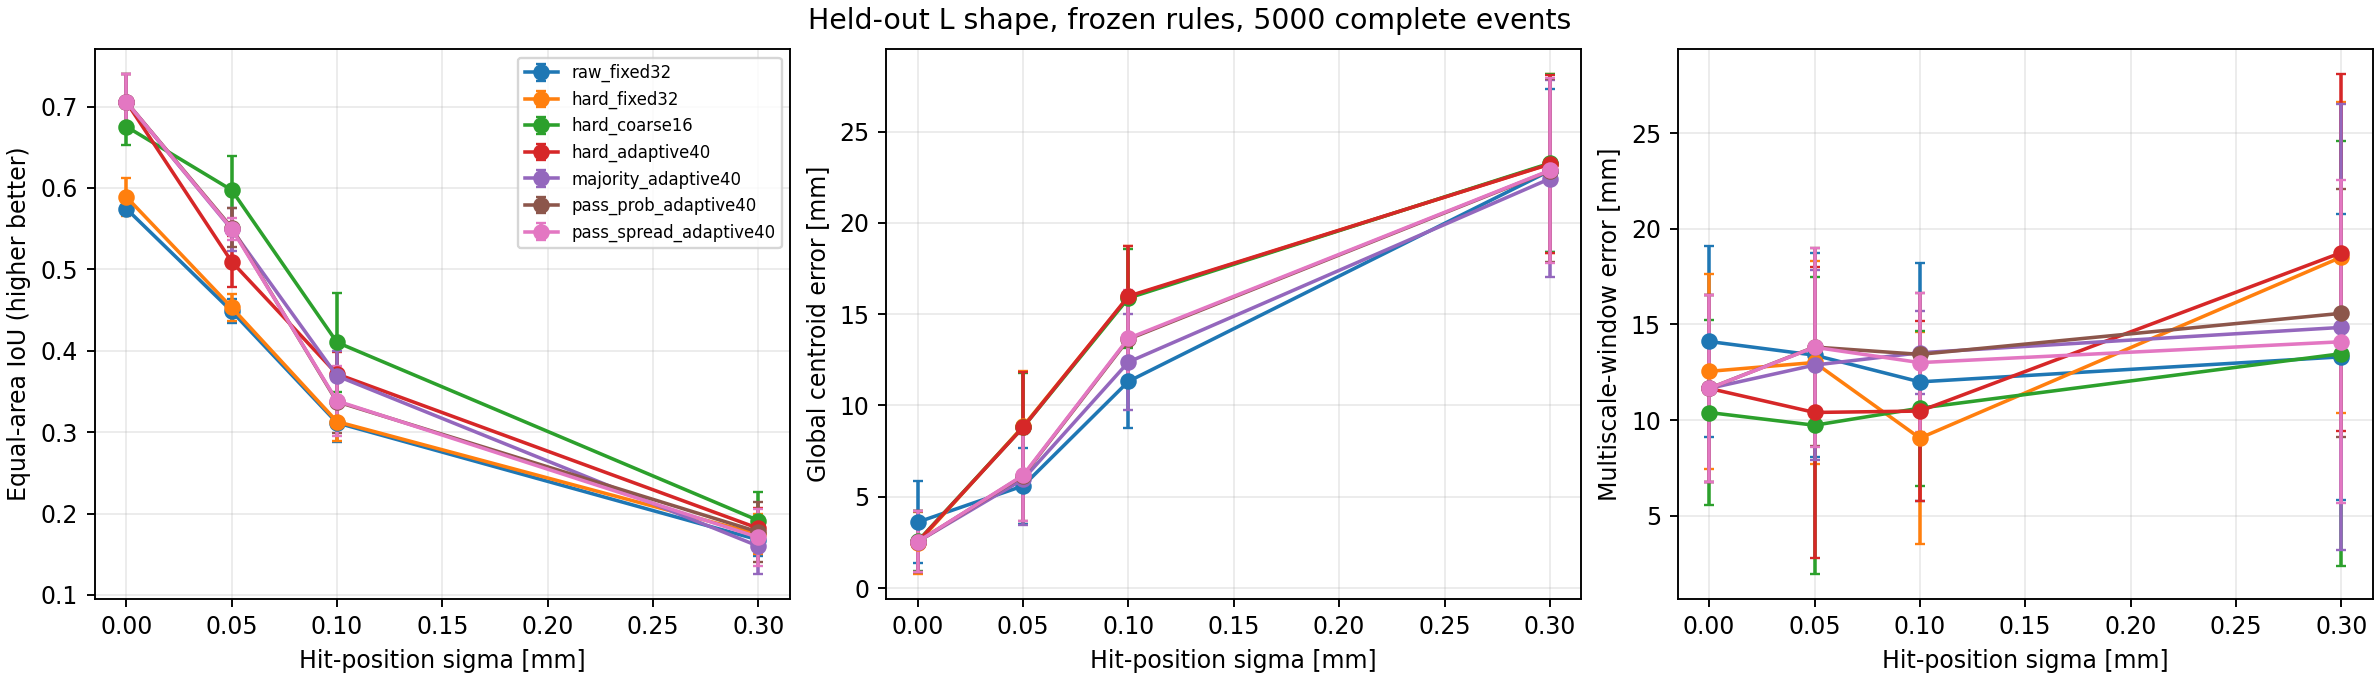
\includegraphics[width=0.95\linewidth]{heldout_l_shape_5000.png}
\caption{留出 L 型目标、$N=5000$ 时的固定规则比较。左列为等面积 IoU，中列为全图质心误差，右列为多尺度自动窗口误差；误差条为 5 次抽样的标准差，而非独立装置重复的置信区间。}
\label{fig:heldout-l-metrics}
\end{figure}

\begin{figure}[htbp]
\centering
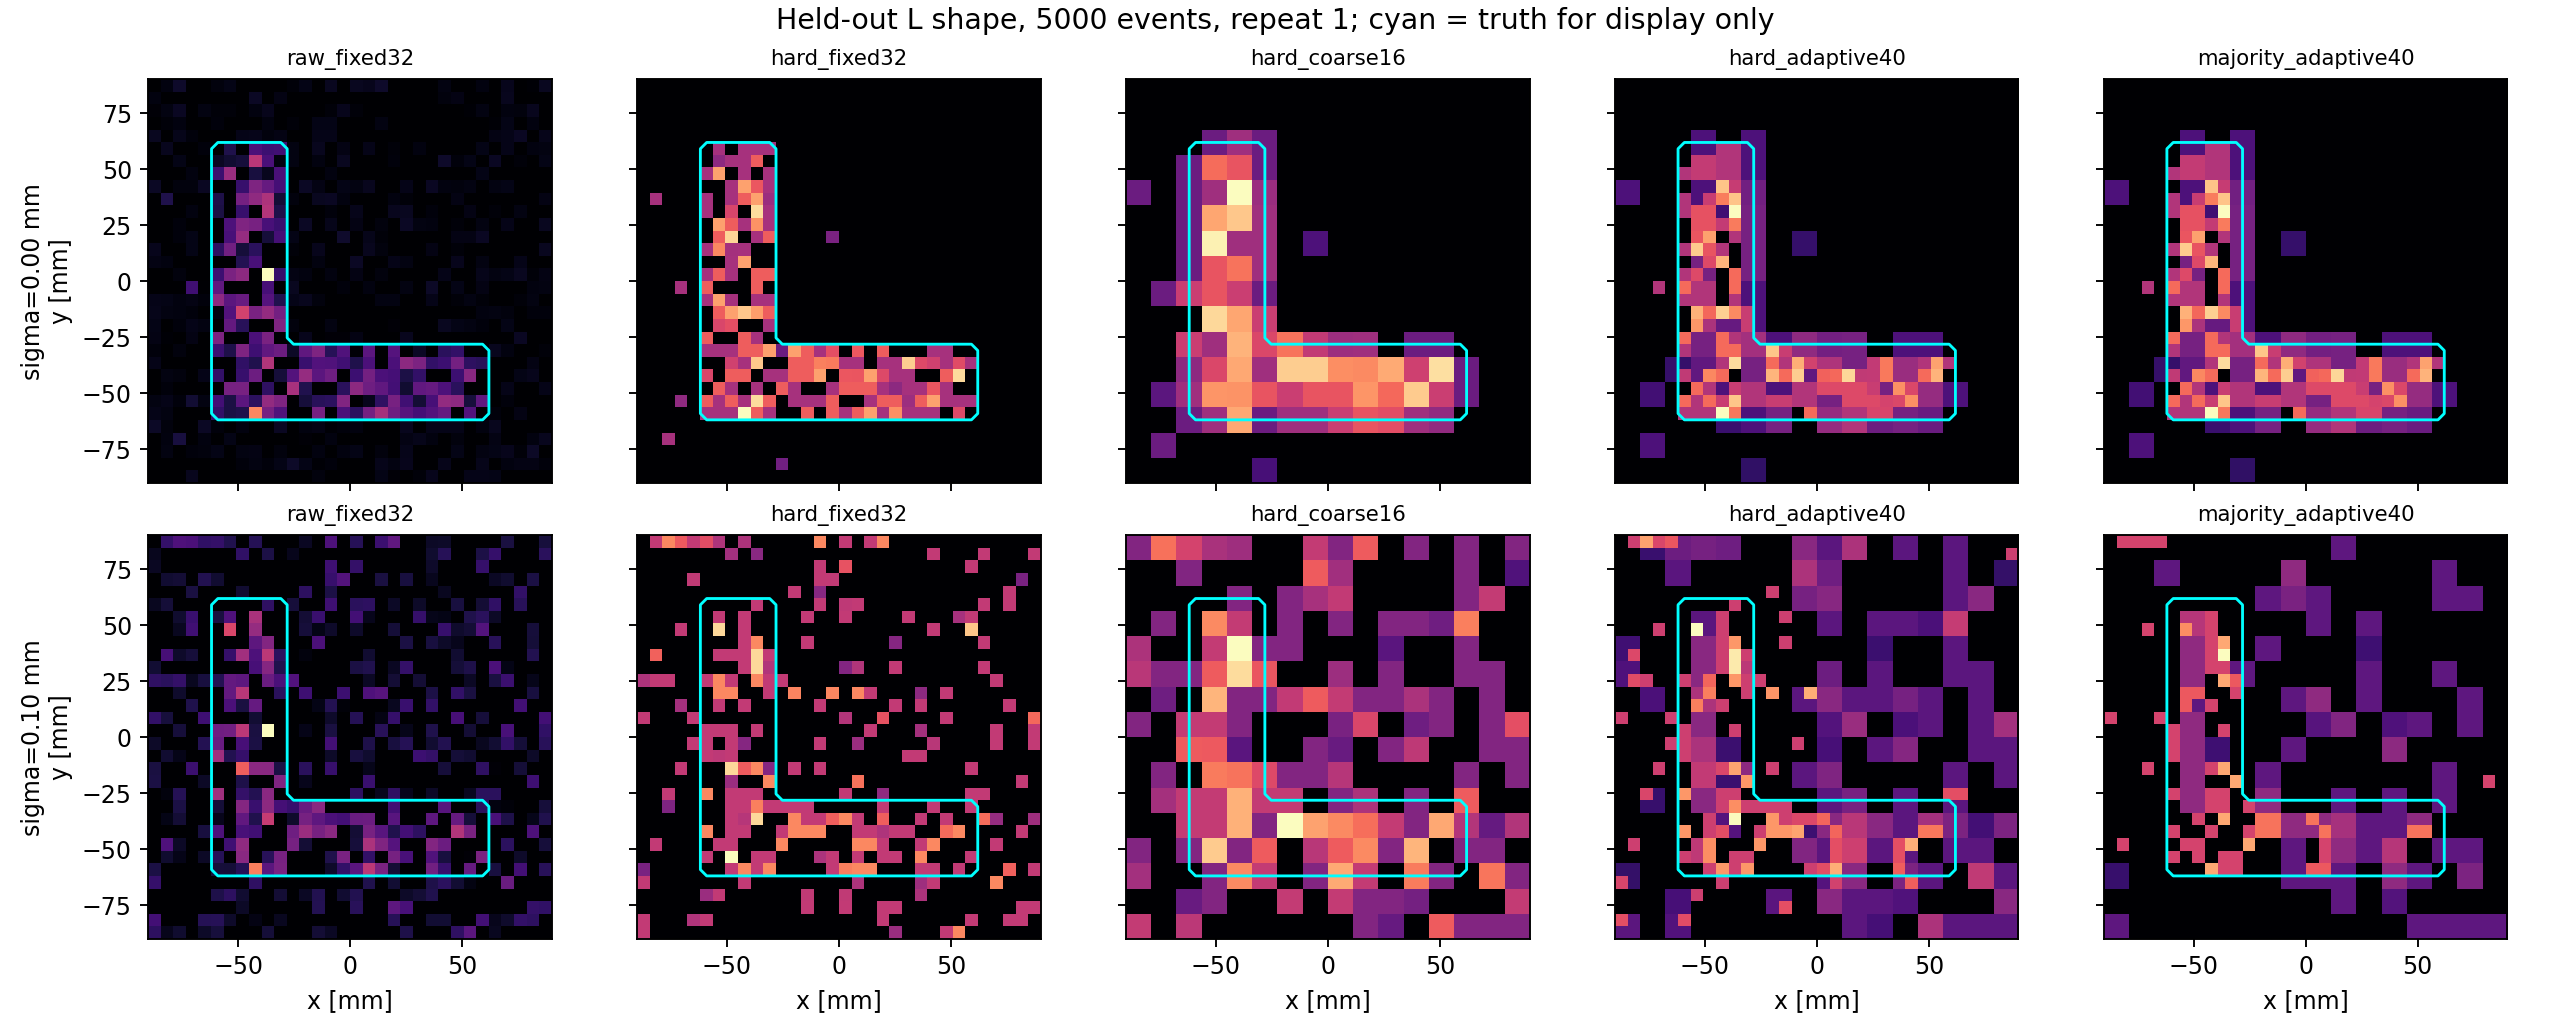
\includegraphics[width=0.98\linewidth]{heldout_l_shape_reconstruction.png}
\caption{L 型目标的代表性 $xy$ 重建图（$N=5000$，第 1 次抽样）。上排为理想击中，下排为 $\sigma=\SI{0.10}{mm}$；青色轮廓仅作真值参考。各面板独立归一化，故只宜比较结构与背景分布。}
\label{fig:heldout-l-images}
\end{figure}

\section{讨论}
\subsection{哪些结果已经得到支持}
现有实验表明，低统计量下固定细体素 POCA 的轮廓恢复明显退化；同一理想源数据上，角度筛选与截断权重可减轻极端大角度事件对重心的影响；把统计量先聚合到粗网格，再局部细分高分数区域，对中心 U 型目标的等面积 IoU 有进一步收益。这个收益并非每个指标都单调改善，低事件数时更多细分可能损失稳定性。探测器位置误差还会同时扰动角度和 POCA，说明仅优化体素参数不足以保证非理想条件下的鲁棒性。留出 L 型目标表明，$40\%$ 细分在理想击中下的轮廓收益不能直接迁移到有噪声测量；粗网格在所测非零误差条件下更稳，支持继续研究由事件统计量与测量误差共同控制的分辨率选择，但尚未构成新规则的验证。事件质量配对实验进一步显示，majority 的平均轮廓收益并不能自动转化为更稳的局部定位；定位器消融揭示了窗口选择本身的误差尾部。因此，事件质量估计、图像轮廓与局部目标定位应分别优化与报告，避免以单一 IoU 作为全部成像任务的替代指标。

\subsection{方法学限制与当前不能做的推断}
第一，角度阈值、上限和细分比例均在有限中心场景中扫描；尽管加入一个未参与原有规则选择的 L 型目标，测试仍只覆盖两类铝目标，且装置与理想源未变化，不能据此宣称跨材料或任意形状泛化。第二，等面积 Top-k IoU 依赖真值目标面积，只适用于当前受控仿真评分。第三，数据来自理想化入射与探测器配置，未建立真实宇宙线通量、动量测量、探测效率及本底；输入事件数不能直接换算为实际测量时间。第四，当前 $16^3$ 到 $32^3$ 的一层细分仍会映射到规则网格计算 IoU，计算代价、内存及可扩展性需要与更严格的对照一起报告。第五，POCA 的单点近似及图像强度的角度平方求和不等于材料散射密度的定量反演。第六，12 次测量值再扰动产生的 $p_i$ 和 $s_i$ 依赖给定的 $\sigma$ 和简化独立高斯误差假设，不能当作已标定探测器的真实通过概率。第七，固定 24 格窗口含目标尺度先验，窗口触边仅为风险信号；事后选出的失败图不构成方法改进的独立证据。第八，L 型场景的重复来自同一份 Geant4 数据的抽样；如果将来依据本轮 L 型结果设计新规则，就不能再把同一 L 型数据作为该新规则的未见测试集。

\subsection{下一阶段的独立验证}
下一阶段宜在开发场景中构造不读取目标真值的细分规则，使局部事件计数、观测散射强度与探测器误差共同决定是否继续细分；固定规则后须另用\emph{新的}目标形状或材料检验，而不能在 L 型结果上调参后继续把 L 型称作留出测试。同时保留同筛选条件下的固定粗、固定细、仅角度修正和联合方法消融。针对窗口失败，应预先规定不使用真值的风险判据与回退策略，然后在全新场景评价平均误差、P90 与失败率，不能以本稿个案倒推调参。对真实未知目标，应增加不依赖真值面积的检测或分割评价流程。机器学习事件质量评分可作为后续辅助模块，但应采用跨场景分组划分数据，且保持与物理基线公平对照，不把它提前写成本稿已完成的结果。

\section{结论}
本文建立了四层探测器、U 型铝目标、事件 CSV 与 Python POCA 重建的可复现工作链路。在理想 \SI{4}{GeV} 平行源下，固定 $32^3$ 体素的等面积 IoU 随输入事件数从 \num{1000} 增至 \num{9975}，由 $0.2836$ 提升至 $0.8409$。在 \num{5000} 条输入事件条件下，角度筛选与截断加权对应的固定细体素 IoU 为 $0.6324$，粗到细、$40\%$ 候选细分时为 $0.7234$。探测器误差实验表明，这些改进对击中位置精度敏感；简化角度噪声扣除不能普遍恢复成像性能。五个 U 型场景的配对比较发现，多数通过筛选对等面积轮廓有平均收益，却未稳定改善自动窗口定位。固定规则在留出 L 型目标上的比较进一步表明，理想击中下 $40\%$ 细分的 IoU 优于粗网格，而在 $\sigma=\SI{0.05}{mm}$ 时粗网格更优。这限制了“固定比例细分普遍有效”的结论，也指出下一阶段应研究误差与统计量共同驱动的分辨率选择，并用未参与规则设计的新场景再次验证。

\bibliographystyle{unsrt}
\bibliography{references}

\clearpage
\section*{工作稿维护清单（投稿前删除）}
\begin{enumerate}[leftmargin=2em]
\item 补充作者单位、通讯作者及基金信息；确定目标期刊后替换为其官方模板。
\item 使用 Zotero 核对并扩充近年方法文献；逐条明确本文与已有大体素、角度截断、事件筛选工作的差异。
\item L 型留出形状已经完成固定参数检查；下一轮仍需新的独立目标形状、不同材料、物理源模型及探测效率验证，不能用同一 L 型数据反复调参和测试。
\item 统一所有实验脚本的随机种子与配对分组，补充置信区间或适当的统计检验。
\item 检查文中每个数值与对应 CSV、图像及代码提交版本一致，再把结果写入摘要。
\item 为真值面积未知的实际成像任务设计可用的阈值和轮廓评价方案。
\item 在未参与筛选、定位器分析的新目标家族中预先固定规则，验证事件质量收益和窗口失效风险；不得把事后挑选的诊断案例当作独立验证。
\end{enumerate}
\end{document}
